\section{Tổng quan về Dữ liệu lớn}

Dữ liệu lớn (Big Data) không đơn thuần chỉ là sự gia tăng về mặt dung lượng lưu trữ, mà là một thuật ngữ bao trùm các tập dữ liệu có kích thước, tốc độ phát sinh và sự đa dạng vượt quá khả năng thu thập, lưu trữ, quản lý và phân tích của các kiến trúc cơ sở dữ liệu truyền thống. Theo định nghĩa của Viện Tiêu chuẩn và Công nghệ Quốc gia Hoa Kỳ (NIST), Big Data đòi hỏi các kiến trúc hệ thống có khả năng mở rộng ngang (horizontal scaling) để phân phối việc xử lý và lưu trữ trên các cụm máy chủ \cite{NIST2015}.

Sự chuyển dịch sang Big Data đánh dấu bước ngoặt từ mô hình tính toán tập trung sang tính toán phân tán (distributed computing), nơi các giải pháp như MapReduce hay Spark đóng vai trò cốt lõi trong việc xử lý song song dữ liệu \cite{Dean2008}.

\vspace{0.5em}
\textbf{Đặc trưng cốt lõi của Dữ liệu lớn (Mô hình 5V)}
\vspace{0.5em}

Mặc dù ban đầu được Doug Laney định nghĩa với mô hình 3V (2001), các nghiên cứu hiện đại đã mở rộng thành mô hình 5V để phản ánh đầy đủ tính chất của dữ liệu lớn trong kỷ nguyên số \cite{Laney2001}:

\begin{itemize}
    \item \textbf{Volume (Dung lượng):} Đề cập đến kích thước khổng lồ của dữ liệu, chuyển từ Terabytes sang Petabytes và Exabytes.
    \item \textbf{Velocity (Tốc độ):} Tốc độ dữ liệu được tạo ra và yêu cầu xử lý theo thời gian thực (Real-time) hoặc gần thời gian thực (Near real-time).
    \item \textbf{Variety (Sự đa dạng):} Sự phong phú của các loại dữ liệu, bao gồm:
    \begin{itemize}
        \item \textit{Dữ liệu có cấu trúc (Structured):} RDBMS, CSV.
        \item \textit{Dữ liệu bán cấu trúc (Semi-structured):} XML, JSON.
        \item \textit{Dữ liệu phi cấu trúc (Unstructured):} Văn bản, video, log hệ thống.
    \end{itemize}
    \item \textbf{Veracity (Tính xác thực):} Đề cập đến độ tin cậy và chất lượng của dữ liệu. Trong môi trường phân tán, dữ liệu thường chứa nhiễu (noise) và cần quy trình làm sạch phức tạp \cite{Wamba2015}.
    \item \textbf{Value (Giá trị):} Khả năng chuyển đổi dữ liệu thô thành thông tin hữu ích hỗ trợ ra quyết định kinh doanh. Đây là mục tiêu cuối cùng của mọi hệ thống Big Data.
\end{itemize}

\subsection{Cơ chế đường ống dữ liệu (Data Pipeline)}

Một hệ thống Big Data hiệu quả không chỉ dựa vào khả năng lưu trữ mà còn phụ thuộc vào quy trình tự động hóa việc luân chuyển và xử lý dữ liệu, được gọi là Data Pipeline. Về bản chất, Data Pipeline là một tập hợp các quy trình tuần tự bao gồm trích xuất (ingestion), xử lý (processing) và lưu trữ dữ liệu, thường được mô hình hóa dưới dạng Đồ thị không chu trình có hướng (Directed Acyclic Graph - DAG) để quản lý sự phụ thuộc giữa các tác vụ \cite{Reis2022}. Mục tiêu tối thượng của đường ống là loại bỏ sự can thiệp thủ công, đảm bảo dữ liệu di chuyển từ nguồn đến đích với độ trễ thấp nhất và tính toàn vẹn cao nhất.

Trong kiến trúc hiện đại, Data Pipeline đã chuyển dịch từ mô hình ETL (Extract-Transform-Load) truyền thống sang mô hình ELT (Extract-Load-Transform) để tận dụng sức mạnh tính toán của các hệ thống lưu trữ phân tán. Hơn nữa, yêu cầu về xử lý dữ liệu không còn giới hạn ở xử lý theo lô (Batch Processing) mà ngày càng hướng tới xử lý dòng (Stream Processing) để đáp ứng nhu cầu phân tích thời gian thực. Theo Martin Kleppmann, một đường ống dữ liệu chuẩn mực phải đảm bảo tính tin cậy (reliability), khả năng mở rộng (scalability) và tính bảo trì (maintainability), cho phép hệ thống tự động phục hồi khi có lỗi xảy ra trong quá trình vận chuyển dữ liệu \cite{Kleppmann2017}.

\subsection{Kiến trúc Data Pipeline Florus}

Được tích hợp vào đồ án này là hệ thống Florus - được xây dựng dựa trên kiến trúc \textbf{Data Lakehouse}, kết hợp tính linh hoạt của Data Lake với khả năng quản lý cấu trúc của Data Warehouse. Hệ thống tuân thủ mô hình \textbf{Medallion Architecture}\footnote{Databricks, ``What is a Medallion Architecture?,'' 2023. Truy cập: \url{https://www.databricks.com/glossary/medallion-architecture}} (Bronze, Silver, Gold) để chuẩn hóa dữ liệu qua từng bước xử lý. Toàn bộ hệ thống được triển khai trên hạ tầng phân tán gồm 7 node vật lý, đảm bảo khả năng sẵn sàng cao và khả năng giám sát.

% Cấp con đầu tiên
\subsubsection{Hạ tầng Phân tán}
Hệ thống được triển khai trên cụm 7 node (BDNode1 - BDNode7) với sự phân chia vai trò cụ thể để tối ưu hiệu năng và tài nguyên:

\begin{itemize}
    \item \textbf{Resource Intensive Nodes (BDNode1 - BDNode4):} 
    \begin{itemize}
        \item Chuyên trách các tác vụ nặng về tính toán và lưu trữ như HDFS (Lưu trữ phân tán) và YARN (Quản lý tài nguyên).
        \item Các Spark Workers được phân bố đều tại đây để thực hiện xử lý song song.
    \end{itemize}
    \item \textbf{Service Nodes (BDNode5 - BDNode7):}
    \begin{itemize}
        \item \textbf{BDNode5:} Chứa Visualization Service (Apache Superset) và cụm Kafka Brokers.
        \item \textbf{BDNode6:} Chứa Delta Service và API Gateway.
        \item \textbf{BDNode7:} Chứa Auth Service, Ingestion Service, Model Service, Serving Service và MongoDB Primary Node.
    \end{itemize}
    \item \textbf{High Availability Cluster:} HDFS được cấu hình HA với Zookeeper, bao gồm Active NameNode và Standby NameNode để tự động chuyển đổi dự phòng khi có sự cố, đảm bảo hệ thống luôn hoạt động.
\end{itemize}

% Cấp con thứ hai
\subsubsection{Chi tiết Các Tầng Chức năng}
Hệ thống được chia thành 5 tầng logic chính, xử lý dòng chảy của dữ liệu từ nguồn đến người dùng cuối.

% Sử dụng paragraph cho các tầng để phân biệt rõ nhưng vẫn nằm trong subsubsection
\paragraph{Tầng Thu thập Dữ liệu (Data Ingestion Layer)}
\mbox{}\\
Tầng này chịu trách nhiệm đưa dữ liệu vào hệ thống từ nhiều nguồn khác nhau (IoT, Database, Files) thông qua hai phương thức chính:

\begin{itemize}
    \item \textbf{Streaming Ingestion (Xử lý luồng):}
    \begin{itemize}
        \item \textbf{Công nghệ:} Apache Kafka, Kafka Connect, Schema Registry.
        \item \textbf{Cơ chế:} Thu thập dữ liệu thời gian thực từ MQTT (cảm biến IoT), MySQL, PostgreSQL (CDC).
        \item \textbf{Stream Validation:} Sử dụng \textit{Kafka Single Message Transform (SMT)} để lọc và kiểm tra dữ liệu ngay trên luồng trước khi lưu trữ (ví dụ: loại bỏ bản tin lỗi, lọc trường dữ liệu không cần thiết).
        \item \textbf{Dynamic Schema:} Schema Registry tự động suy luận và quản lý phiên bản cấu trúc dữ liệu, hỗ trợ chuyển đổi byte array từ MQTT sang JSON.
    \end{itemize}
    
    \item \textbf{Batch Ingestion (Xử lý lô):}
    \begin{itemize}
        \item \textbf{Công nghệ:} Apache Spark Structured Streaming, Flask (Asyncio).
        \item \textbf{Media Batch Feature:} Tính năng mới cho phép thu thập hàng loạt tệp phi cấu trúc (ảnh, video, PDF, CSV) từ các nguồn Cloud Storage như Google Drive, AWS S3, Azure Blob Storage.
        \item \textbf{Xử lý tệp:} Tệp văn bản (CSV, Excel) được xử lý và lưu vào HDFS để tạo bảng Delta; tệp nhị phân (Ảnh, Video) được lưu trực tiếp vào MinIO.
    \end{itemize}
\end{itemize}

\paragraph{Tầng Lưu trữ (Data Storage Layer)}
\mbox{}\\
Tầng này quản lý việc lưu trữ dữ liệu đa định dạng và metadata, đóng vai trò là trung tâm dữ liệu của hệ thống:

\begin{itemize}
    \item \textbf{HDFS (Hadoop Distributed File System):}
    \begin{itemize}
        \item Lưu trữ các bảng dữ liệu chính dưới định dạng \textbf{Delta Lake}.
        \item \textit{Bronze Table:} Dữ liệu thô vừa được thu thập.
        \item \textit{Silver Table:} Dữ liệu đã làm sạch, chuẩn hóa và biến đổi.
        \item \textit{Gold Table:} Dữ liệu tinh gọn, đã tổng hợp, sẵn sàng cho Analytics/ML.
    \end{itemize}
    \item \textbf{MongoDB:}
    \begin{itemize}
        \item Lưu trữ metadata của hệ thống (User, Project, Configurations).
        \item \textbf{Caching Mechanism:} Cache dữ liệu bảng Silver/Gold (dưới 10,000 dòng) để tăng tốc độ truy vấn xem trước trên UI mà không cần kích hoạt Spark job.
    \end{itemize}
    \item \textbf{MinIO (Object Storage):} Lưu trữ các artifacts của mô hình ML (MLflow artifacts), biểu đồ đã render, và các tệp phi cấu trúc.
    \item \textbf{PostgreSQL:} Kho dữ liệu trung gian để đồng bộ dữ liệu từ HDFS phục vụ cho Apache Superset (giải quyết hạn chế đọc trực tiếp Delta Lake của Superset).
\end{itemize}

\paragraph{Tầng Xử lý \& Phân tích (Processing \& Analytics Layer)}
Thực hiện các tác vụ tính toán, biến đổi dữ liệu và huấn luyện mô hình máy học:

\begin{itemize}
    \item \textbf{Data Processing (ETL):}
    \begin{itemize}
        \item \textit{Apache Spark:} Engine chính xử lý dữ liệu phân tán.
        \item \textit{Query Builder:} Cung cấp giao diện Visual Query (kéo thả) và SQL Editor để người dùng truy vấn dữ liệu ad-hoc và tạo bảng mới từ kết quả truy vấn.
    \end{itemize}
    \item \textbf{Machine Learning Engine:}
    \begin{itemize}
        \item \textit{Data Preparation:} Tích hợp các thuật toán tiên tiến như \textbf{cGAN} để điền dữ liệu khuyết và lọc nhiễu.
        \item \textit{Model Training:} Hỗ trợ đa dạng thuật toán từ cơ bản (Linear Regression) đến Deep Learning (ANN, RNN, LSTM, CNN\_LSTM).
        \item \textit{Hyperparameter Tuning:} Tích hợp \textbf{Optuna} để tự động tối ưu hóa tham số mô hình.
    \end{itemize}
\end{itemize}

\paragraph{Tầng API \& Quản lý (API \& Metadata Layer)}
\mbox{}\\
Tầng này đóng vai trò cầu nối, bao gồm các Backend Services được xây dựng bằng \textbf{Flask} và hệ thống quản lý MLflow. Các Backend Services được chia thành 4 microservices chuyên biệt:

\begin{enumerate}
    \item \textbf{Ingestion Service (Dịch vụ Thu thập):}
    \begin{itemize}
        \item Quản lý yêu cầu thu thập (Batch/Stream).
        \item Tương tác với Kafka để cấu hình luồng và luật kiểm tra (Rules).
        \item Kích hoạt Spark để đọc/ghi dữ liệu vào HDFS.
    \end{itemize}
    
    \item \textbf{Delta Service (Dịch vụ Quản lý Dữ liệu):}
    \begin{itemize}
        \item Quản lý vòng đời các bảng Delta (Bronze/Silver/Gold).
        \item Xử lý truy vấn dữ liệu thông qua cơ chế Caching thông minh.
        \item Cung cấp \textbf{Access Token} cho các hệ thống bên ngoài truy xuất dữ liệu an toàn qua API.
    \end{itemize}
    
    \item \textbf{Model Service (Dịch vụ Huấn luyện):}
    \begin{itemize}
        \item Quản lý quy trình chuẩn bị dữ liệu và huấn luyện.
        \item Tương tác với \textbf{MLflow Tracking} để ghi nhận metrics, params.
        \item Quản lý \textbf{Optuna} cho việc tối ưu tham số.
    \end{itemize}
    
    \item \textbf{Serving Service (Dịch vụ Triển khai):}
    \begin{itemize}
        \item Tự động hóa việc đóng gói mô hình thành \textbf{Docker Container}.
        \item Quản lý triển khai container lên hạ tầng (AWS Fargate/Docker).
        \item Định tuyến yêu cầu dự báo đến đúng container mô hình.
    \end{itemize}
\end{enumerate}

Ngoài ra, tầng này còn chứa \textbf{MLflow} để quản lý vòng đời MLOps (Tracking \& Model Registry).

\paragraph{Tầng Tiêu thụ \& Trực quan hóa (Consumption Layer)}
\mbox{}\\
Tầng này cung cấp giao diện tương tác cuối cùng dành cho người dùng:

\begin{itemize}
    \item \textbf{Data Visualization (Apache Superset):} Tích hợp sâu vào hệ thống, cho phép tạo Dashboard tương tác, nhiều loại biểu đồ (Heatmap, Bar, Line, Deck.GL Geo-spatial) với cơ chế phân quyền (RBAC) đồng bộ.
    \item \textbf{Model Serving (Containerization):} Mỗi mô hình đã huấn luyện được đóng gói thành một \textbf{Docker Container} độc lập, cung cấp REST API riêng biệt (/predict) để dự báo thời gian thực.
\end{itemize}

% Cấp con thứ ba (ngang hàng với Chi tiết các tầng)
\subsubsection{Hệ thống Giám sát (Monitoring System)}
Florus 3.0 tích hợp giải pháp giám sát toàn diện để đảm bảo độ tin cậy và khả năng quan sát:

\begin{itemize}
    \item \textbf{cAdvisor:} Thu thập metrics thời gian thực (CPU, RAM, Network) từ tất cả các Docker container, bao gồm các Services nền tảng và các Model Serving container.
    \item \textbf{JMX Exporter:} Giám sát các thành phần Java-based như Hadoop Cluster (NameNode, DataNode) và Kafka Brokers.
    \item \textbf{Prometheus:} Cơ sở dữ liệu Time-series để lưu trữ và truy vấn metrics thu thập được.
    \item \textbf{Grafana:} Hiển thị Dashboard giám sát sức khỏe toàn hệ thống (Node health, Service status, Resource usage).
    \item \textbf{Health-check APIs:} API tích hợp sẵn trong từng microservice để kiểm tra trạng thái sống (Liveness probes), cho phép hệ thống tự động phát hiện sự cố.
\end{itemize}

% \clearpage
% \newgeometry{top=0cm, bottom=0cm, left=4cm, right=0cm} % Ép lề nhỏ lại chỉ cho trang này
% \begin{landscape}
%     \thispagestyle{plain} % Bỏ Header "Đồ án...", chỉ giữ số trang ở dưới footer (tùy chọn)
    
%     \begin{figure}[H]
%         \centering
%         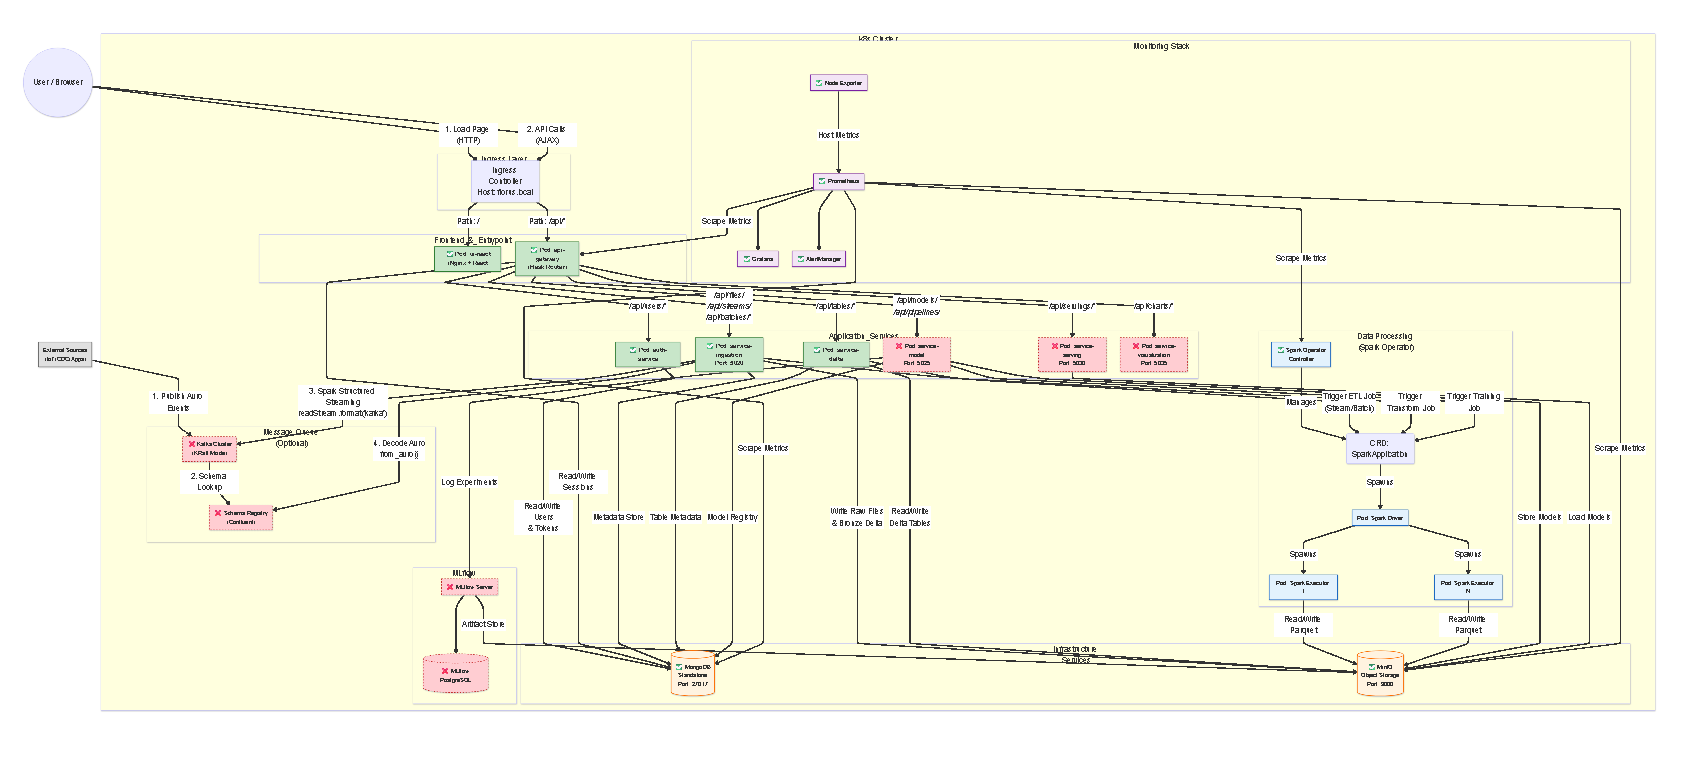
\includegraphics[width=1.0\linewidth, height=1.0\textheight, keepaspectratio]{images/chap 3/florus-full-lr (1).pdf}
%         \caption{Kiến trúc triển khai hệ thống Florus trên nền tảng Kubernetes}
%         \label{fig:florus-arch}
%     \end{figure}
% \end{landscape}
% \restoregeometry % Trả lại lề chuẩn cho các trang sau
\clearpage
\newgeometry{top=0cm, bottom=0cm, left=4cm, right=0cm} % Ép lề nhỏ lại chỉ cho trang này
\begin{landscape}
    \thispagestyle{plain} % Bỏ Header "Đồ án...", chỉ giữ số trang ở dưới footer (tùy chọn)
    
    \begin{figure}[H]
        \centering
        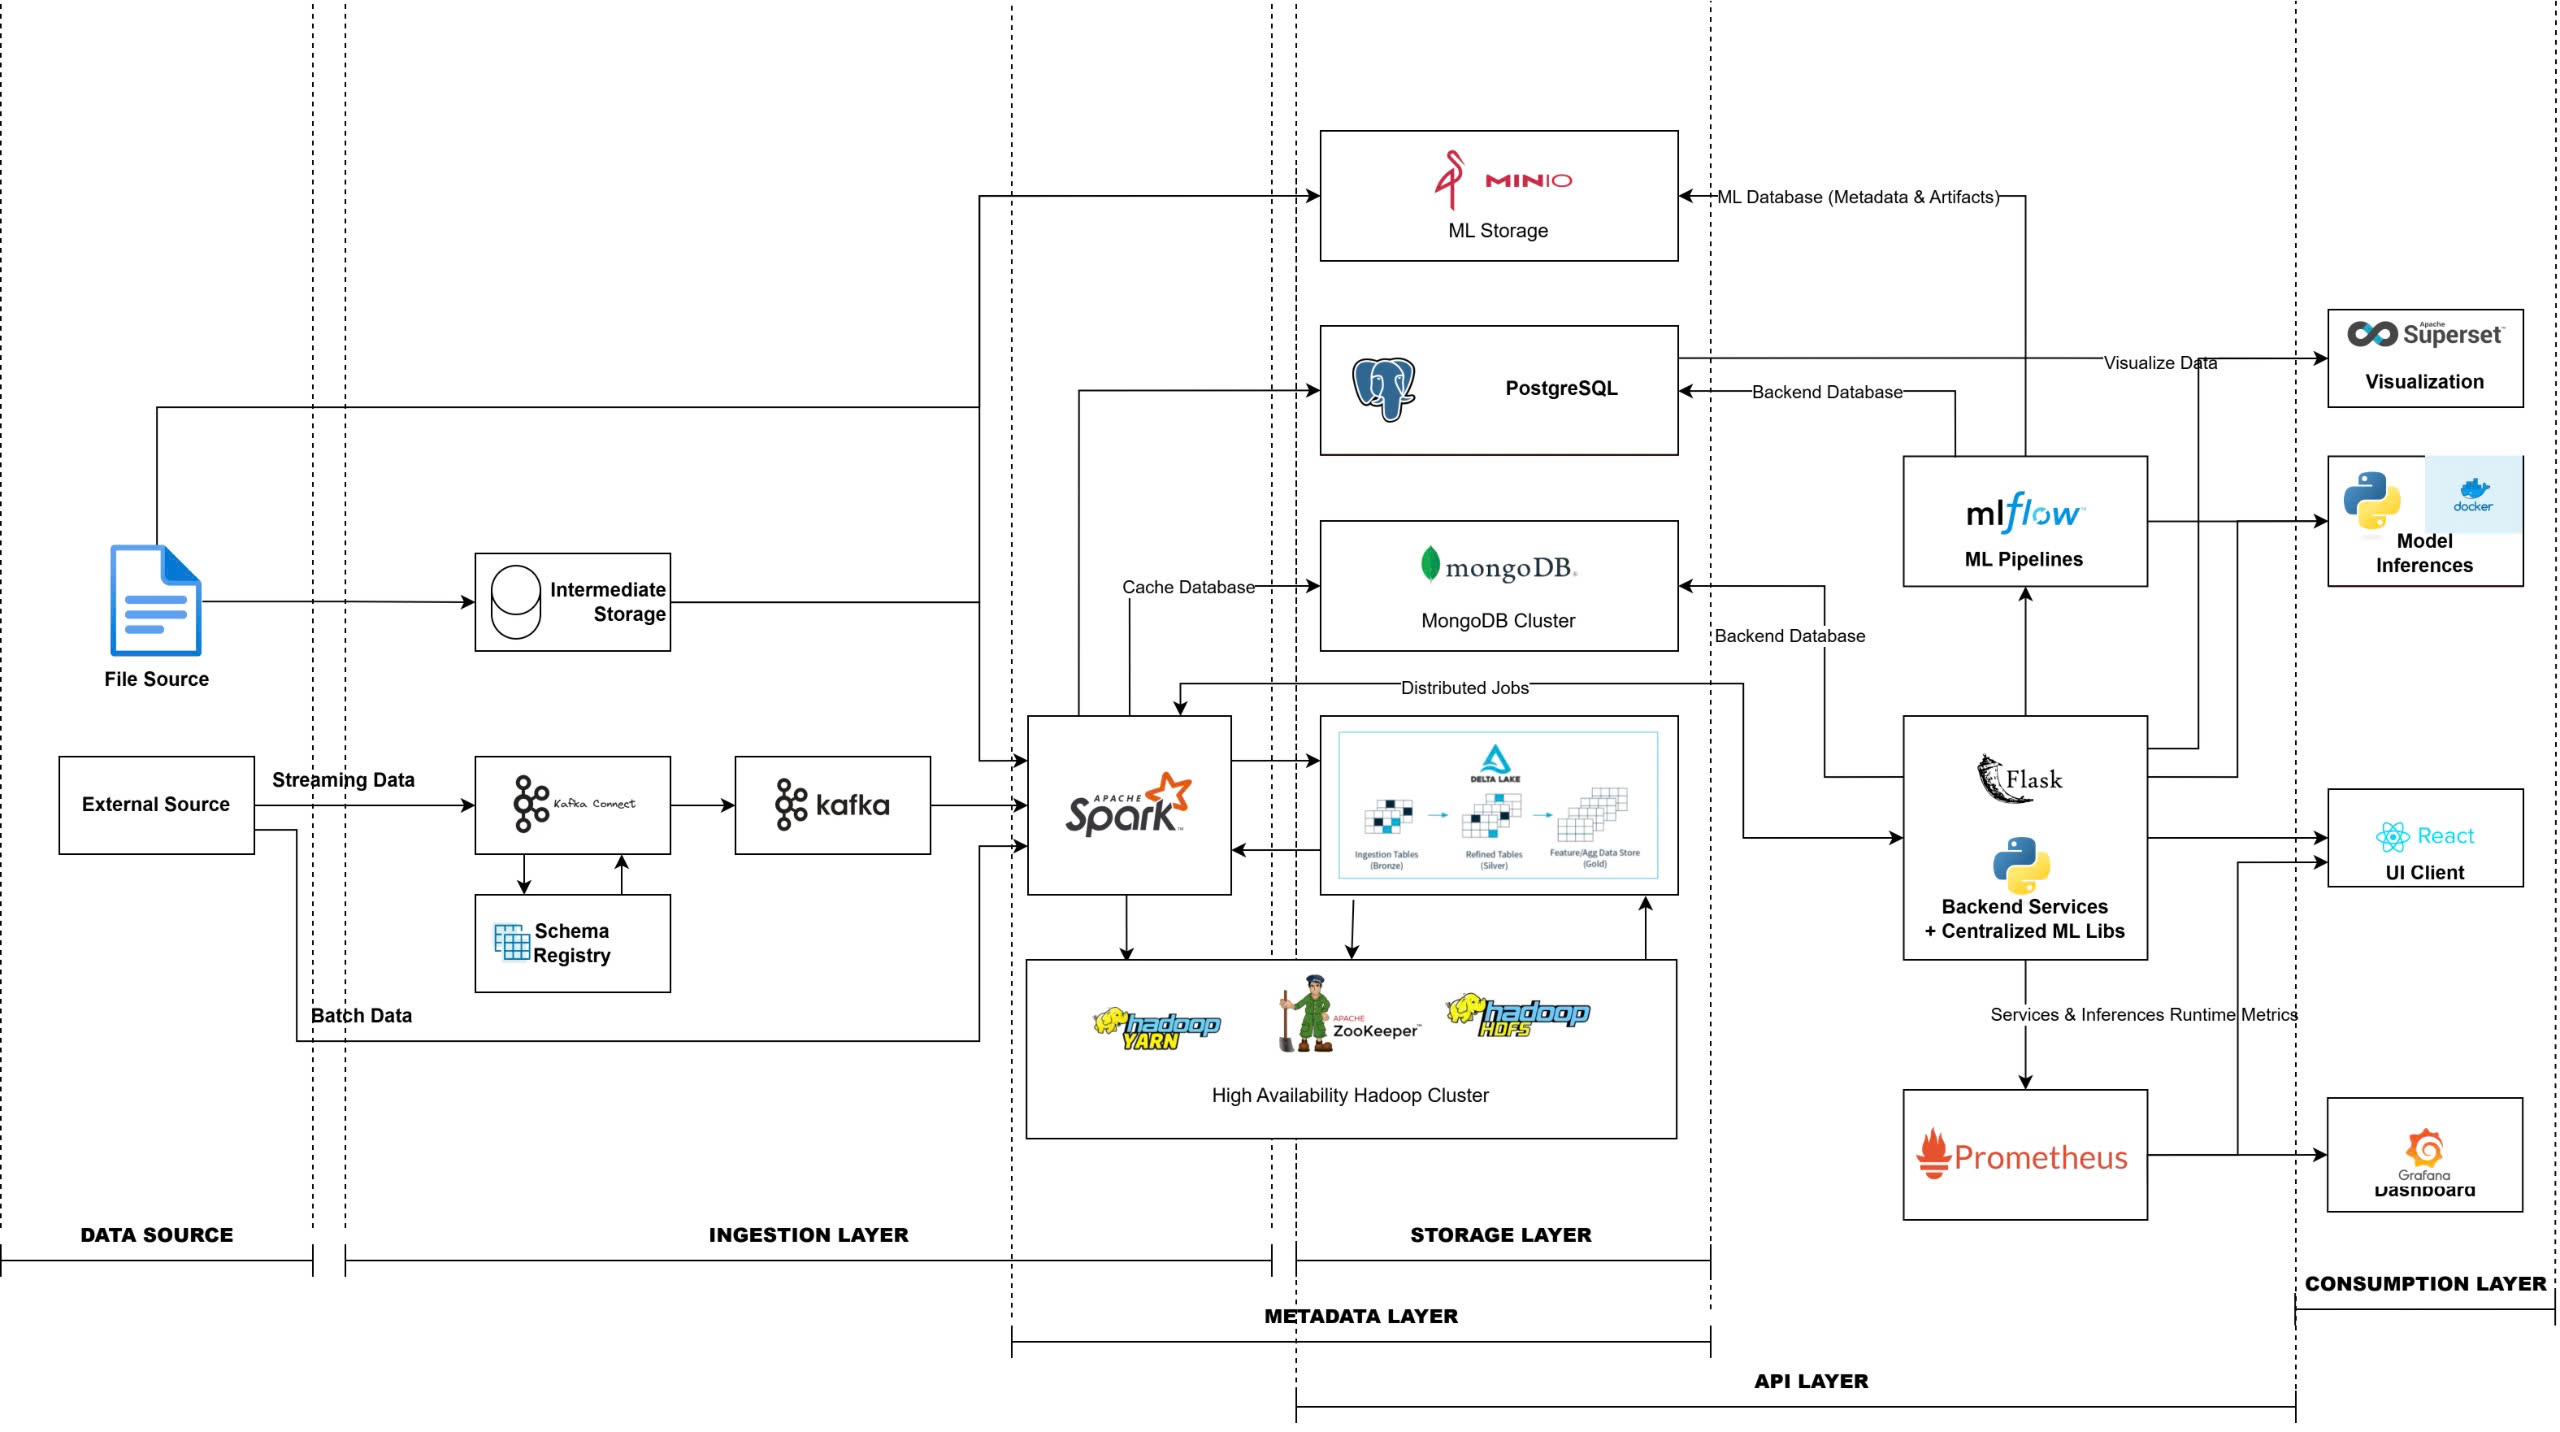
\includegraphics[width=0.9\linewidth, height=1.0\textheight, keepaspectratio]{images/chap 2/florus-arch.jpg}
        \vspace{2em}
        \caption{Kiến trúc hệ thống Florus}
        \label{fig:florus-arch}
    \end{figure}
\end{landscape}
\restoregeometry % Trả lại lề chuẩn cho các trang sau
% \begin{figure}[H]
%     \centering
%     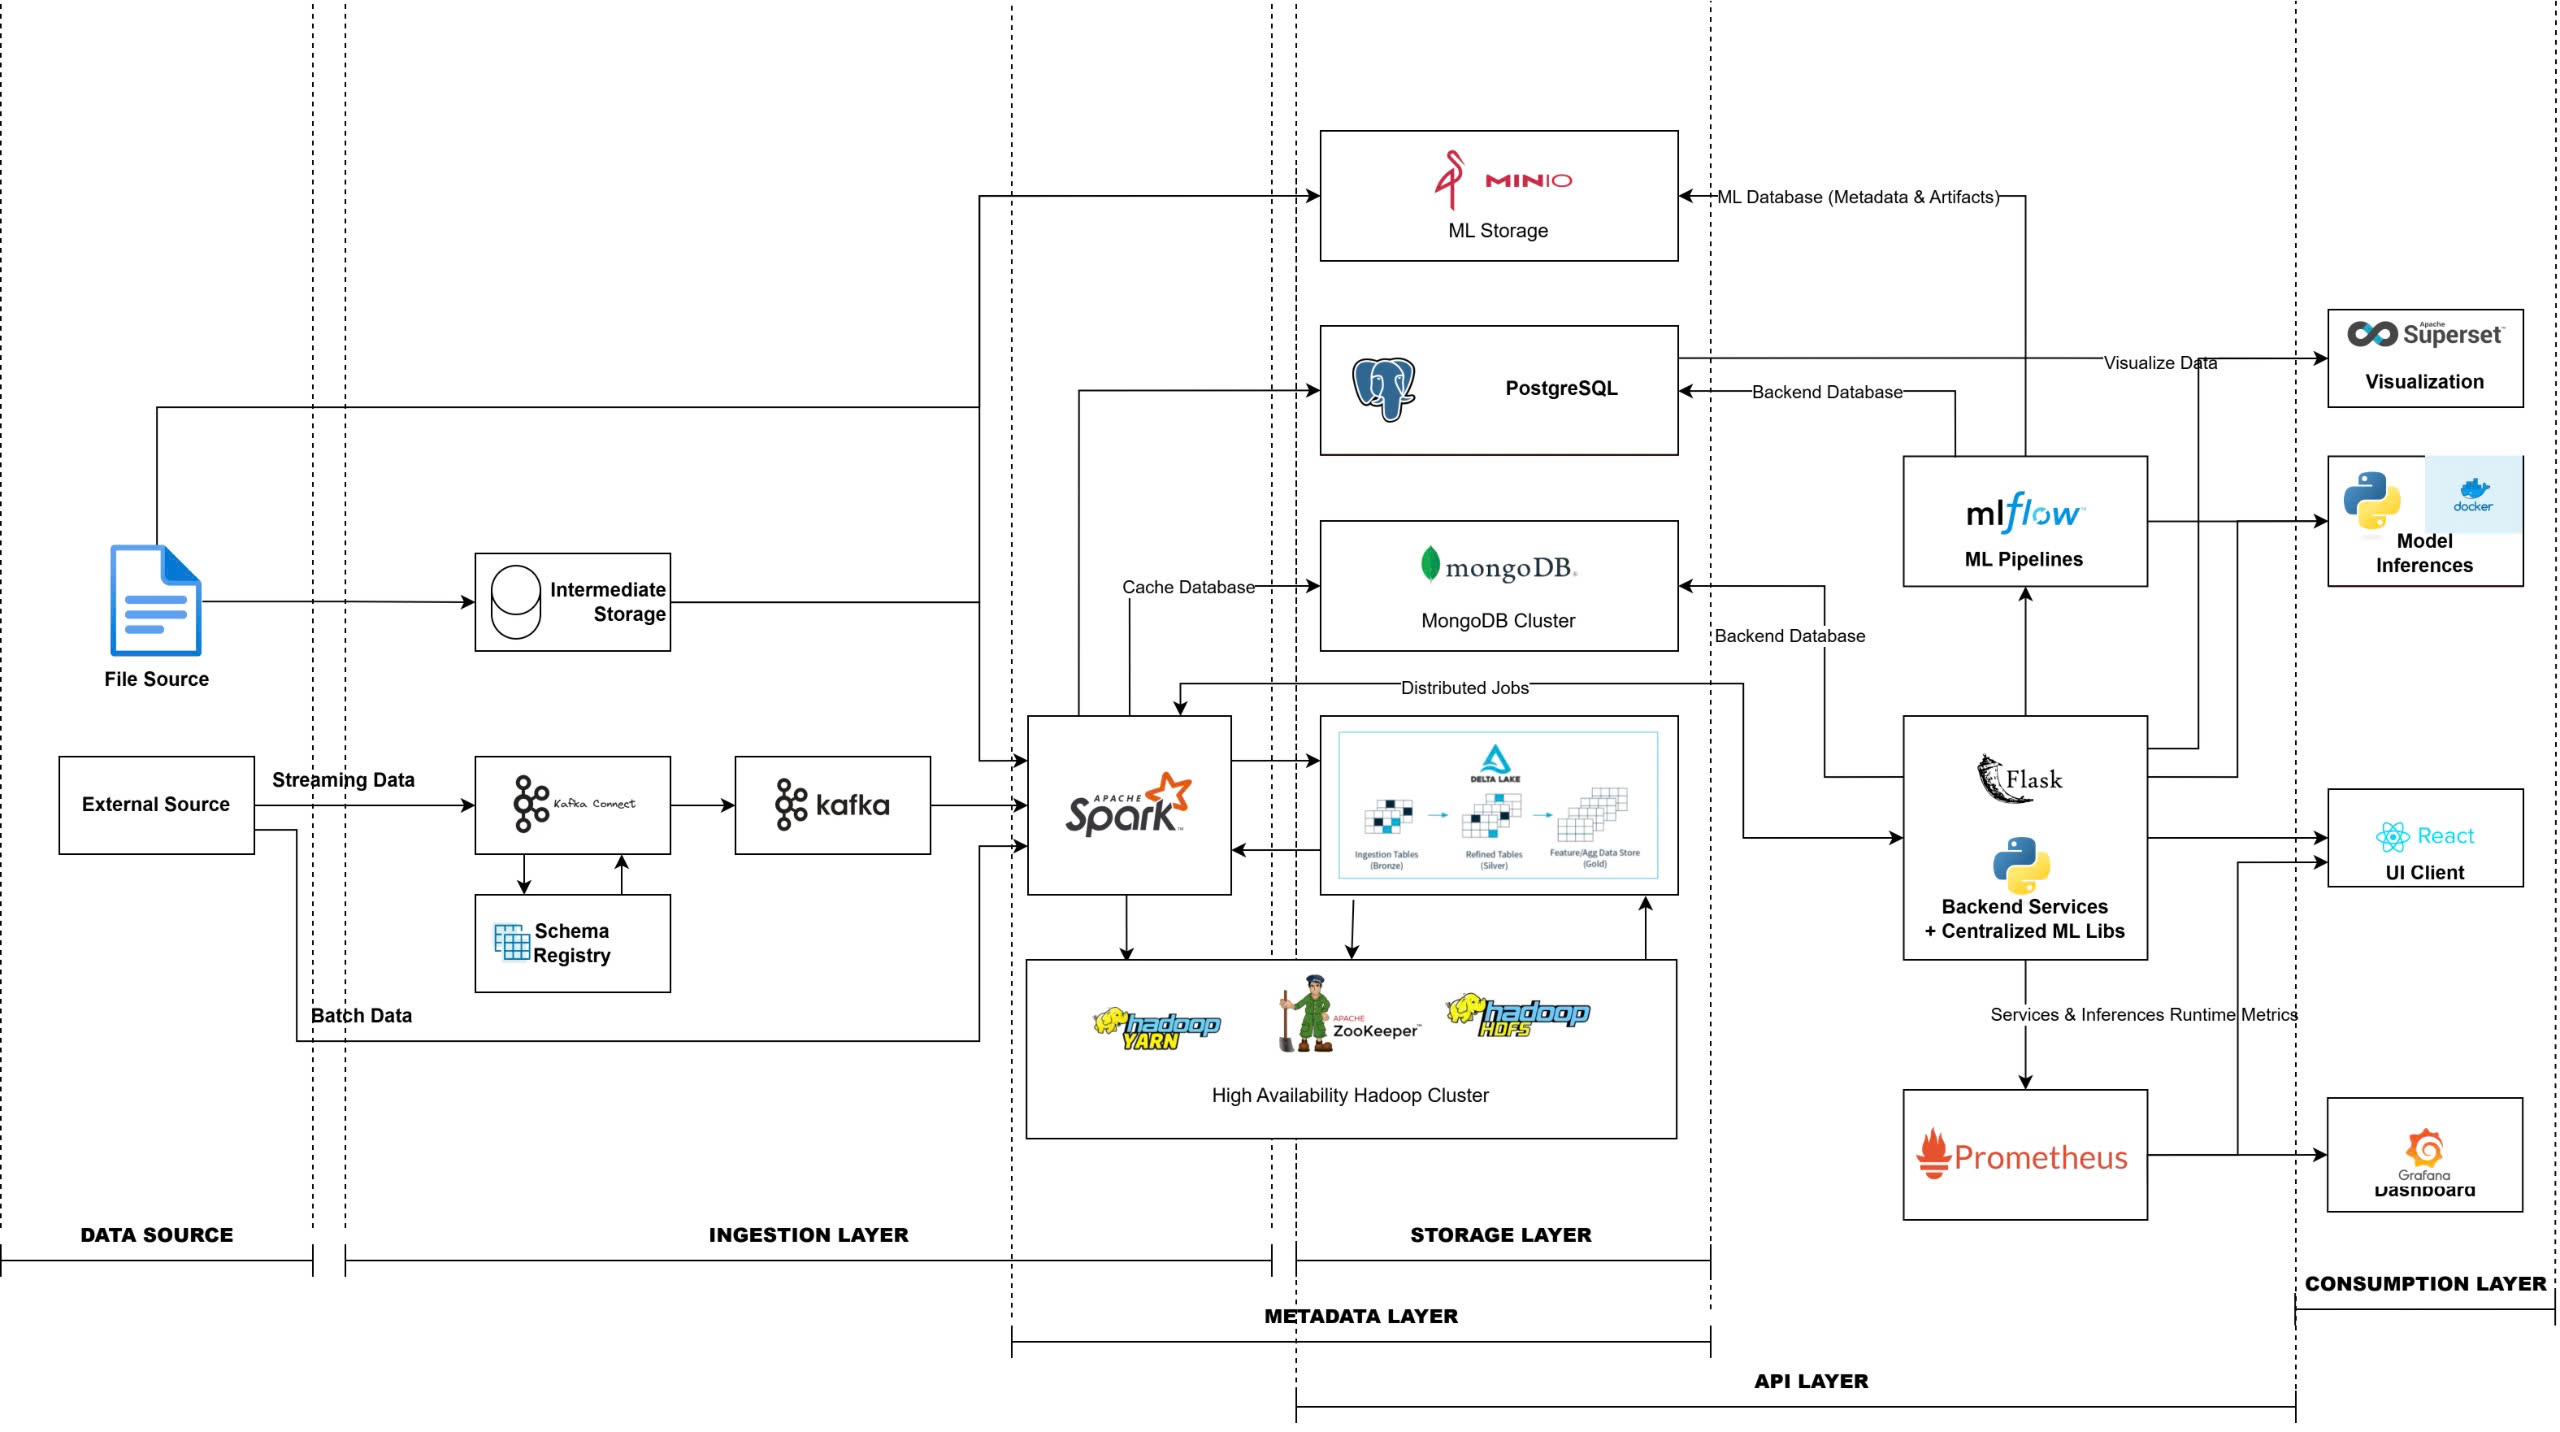
\includegraphics[width=1\linewidth]{images/chap 2/florus-arch.jpg}
%     \vspace{2em}
%     \caption{Kiến trúc hệ thống Florus}
% \end{figure}